\documentclass[11pt]{article}
\usepackage[utf8]{inputenc}
\usepackage[T1]{fontenc}
\usepackage{babel}
\usepackage{graphicx}
\usepackage{xcolor}
\usepackage{listings}
\usepackage[colorlinks=true,linkcolor=blue, urlcolor=blue]{hyperref}


\lstset{
    basicstyle=\ttfamily,
    backgroundcolor=\color{lightgray},
    frame=single,
    columns=flexible
}

\date{Version Mai 2024}
\author{Valentin Gangloff
\and
Master Sécurité des Systèmes Informatiques 1ère année
\and
UFR Sciences et techniques de Rouen}
\title{Guide d'installation du simulateur Mermin}

\begin{document}

\maketitle

\newpage 

\tableofcontents

\newpage

\section{Présentation de l'appareil}

\subsection{Introduction}

Ce guide d'installation est là pour vous présenter le fonctionnement sommaire et les procédures pour construire et configurer l'appareil, dans le cadre du projet de fin d'année conjoint entre le Master SSI et le Master GIL de l'UFR Sciences et Techniques de Rouen.
\\
Le but du projet est de créer un atelier avec, une animation ludique pour permettre à des lycéens de découvrir des propriétés inhérentes à l'informatique quantique.
\\

\noindent Le phénomène principalement retenu est l'intrication quantique dans le cadre du jeu du Carré de Mermin-Peres\footnote{Jeu introduit par Cabello et Aravind sur la base de la pseudo-télépathie quantique de Mermin et Peres}.

\noindent Il a donc été conçu un appareil permettant de remettre en place l'expérience de la pseudo-télépathie quantique.

\subsection{Description de l'appareil}

L'ensemble de l'appareil est composé de 3-4 parties :

\begin{itemize}
	\item D'une interface pour le joueur Alice
	\item D'une interface pour le joueur Bob
	\item D'une unité de contrôle et de calcul qui fonctionne sans fil (Que l'on doit cacher)
	\item D'une troisième interface pour l'unité de contrôle, pour le démarrage (Dont on peut se débarrasser aussitôt après activation)
\end{itemize}

\noindent Sans expliquer le jeu, le fonctionnement externe est sommaire :

Un utilisateur Alice ou Bob, va appuyer sur un bouton sur son interface, et l'appareil affiche une mesure correspondante à la case identifiée par le bouton appuyé.
Cette mesure aura été faite par l'unité de contrôle et de calcul sans fil qui communique en permanence avec les deux interfaces.


\newpage

\subsection{Liste du matériel pour la conception}

La liste du matériel est précise, pour une raison de compatibilité.

L'unité de contrôle est composée d'une unique RaspBerry Pi 5 8Go de dernière génération en Kit de démarrage de chez HutoPi

La liste des composants de l'interface est :
	\begin{itemize}
		\item Deux Arduinos Uno R4 Wi-Fi
		\item Deux écrans LCD tactiles 4D SYSTEMS Gen4-uLCD-43DT de résolution 272x480
		\item Deux Shields de compatibilité arduino / 4D SYSTEMS
		\item D'un adaptateur USB 4D SYSTEMS
		\item D'un lecteur de cartes µSD pour ordinateur
		\item Deux cartes µSD de 4Go minimum
	\end{itemize}
	
\newpage

\section{L'unité de contrôle et de calcul}

\subsection{Présentation de la tâche}

Le but de l'unité de contrôle et de calcul est de contrôler le comportement des Arduinos en communiquant à chaque requête. Elle permet aussi de faire les calculs et les mesures Quantiques associées au jeu, et ce, en temps réel.
\\
\\
Le but a donc été d'en faire un point d'accès Wi-Fi auquel les Arduinos se connectent et sont identifiées, pour communiquer de façon indépendantes l'une de l'autre.
\\
\\
Nous avons donc un fichier gérant les calculs quantiques, un fichier gérant le jeu en général et les Arduinos, et une série de scripts pour faire fonctionner le tout.

\subsection{Mise en place}

\subsubsection{Matériel nécessaire}

Pour l'installation de l'unité de contrôle et de calcul, il vous faut :

\begin{itemize}
	\item Du Kit RaspBerry
	\item D'une alimentation pour la RaspBerry
	\item D'un ordinateur équipé de Linux ou Windows avec transfert SFTP (FileZila est efficace avec Windows)
\end{itemize}

\subsubsection{Initialisation de la RaspBerry}

Récupérez le Kit, montez-le comme il est mentionné dans le mode d'emploi du Kit reçu et lancez le système d'exploitation pour le configurer.

Assurez-vous de mettre à jour le système d'exploitation en ouvrant un terminal et en entrant la commande :

\begin{lstlisting}[language=bash]
	sudo apt update; sudo apt upgrade -y
\end{lstlisting}

\subsubsection{Installation du Hotspot et dépendances}

Pour mettre en place les configurations propices au fonctionnement, déposez le script networksetup.sh n'importe où sur la RaspBerry et lancez-le depuis un terminal :

\begin{lstlisting}[language=bash]
	sudo bash networksetup.sh
\end{lstlisting}

Le script va lancer la réinstallation des locales du système d'exploitation qui peuvent être défectueuses et faire planter le programme.

Il va ensuite installer python et toutes ses dépendances, ainsi que supprimer les warnings de Pip lors de l'installation de bibliothèques python.

Finalement, il va installer les bibliothèques, créer un Hotspot, mettre en place une activation automatique et pour finir, il va activer ce Hotspot.
\\
\\
\textbf{Attention : Si vous êtes connecté en SSH par Wi-Fi sur la RaspBerry, votre connexion sera aussitôt coupée puisque le Hotspot aura prit la place de la connexion initiale de la RaspBerry et ne sera donc plus dans le réseau. Pour continuer, connectez vous tout simplement sur le wifi du RaspBerry}\footnote{SSID : merminrasp, MDP : mermin2024}

\subsubsection{Préparation du programme principal}

Déposez tout simplement le répertoire merminarduino/DeviceCodes/Rasp dans la racine du projet. Pour fonctionner, vous devez avoir à minima un répertoire contenant les fichiers mermingame.py et controller.py et optionnellement le script launch.sh\footnote{Se référer au mode d'emploi pour l'utilité du script}.

L'appareil est donc configuré et prêt à l'emploi, vous pouvez donc vous référer au mode d'emploi pour son utilisation.

\newpage

\section{La carte de contrôle de l'interface}

\subsection{Présentation de la tâche}

Le but de la carte de contrôle et de lire les entrées de l'écran qui sert d'interface, et de communiquer avec l'unité de contrôle et de calcul.
\\
\\
Pour se faire, il faut que la carte puisse se connecter en Wi-Fi sur le Hotspot de la RaspBerry, et communiquer autant avec l'écran connecté qu'avec le Hostpot par connexion socket.

\subsection{Mise en place}

\subsubsection{Matériel nécessaire}

Pour préparer une unique carte, il faut :

\begin{itemize}
	\item Un câble de transfert Data USB-A / USB-C
	\item Un ordinateur avec un OS Linux ou Windows et l'IDE Arduino
	\item La carte Arduino Uno R4 Wi-Fi
	\item Le Shield de compatibilité Arduino / 4D Systems
\end{itemize}

\newpage

\subsubsection{Montage de l'appareil}

Commencez par installer le Shield sur l'Arduino, alignant les pins 0 à AREF comme suit :

\includegraphics[width=\textwidth]{Arduinomonte.jpg}

\noindent Une fois cela fait, branchez le câble USB-C et USB-A à l'Arduino et l'ordinateur pour commencer le transfert du code.

\noindent Ouvrez l'IDE Arduino.

\noindent Pour programmer la carte d'Alice (resp Bob), ouvrez le fichier :

\noindent merminarduino/DeviceCodes/Arduinos/alice.ino 

\noindent(resp merminarduino/DeviceCodes/Arduinos/bob.ino):


\includegraphics[width=\textwidth]{OuvrirArduino.png}

\noindent Ensuite, téléversez-le :


\includegraphics[width=\textwidth]{TeleverserArduino.png}

\noindent Maintenant, l'appareil est prêt à être utilisé, que ça soit pour Alice ou Bob, il vous suffira de brancher l'écran dessus puis, l'alimentation de votre choix.

\newpage

\section{L'écran de l'interface}

\subsection{Présentation de la tâche}

Si l'écran est séparé pour la programmation, c'est à cause de la nature de ce dernier, en effet, pour le programmer et le préparer, il nécessite une attention plutôt particulière.

Le but de l'écran est, d'afficher les mesures, d'afficher la grille des mesures, de faire un retour visuel sur les cases de la grille mesurée et surtout, d'être tactile et donc de détecter les entrées de l'utilisateur.

\subsection{Montage de l'appareil}

\subsubsection{Matériel nécessaire}

Pour préparer un unique écran, il faut :

\begin{itemize}
	\item Une carte d'interface USB / 4D SYSTEMS
	\item Une carte µSD de 4Go minimum
	\item Un écran 4D SYSTEMS Gen4-uLCD-43DT de résolution 272x480
	\item Un câble data USB / Mini USB du début des années 2000
	\item Un ordinateur avec un OS Linux et un OS Windows (Ou une VM avec Windows dessus) et l'\href{https://4dsystems.com.au/software/}{IDE 4D SYSTEMS WorkShop}\footnote{Lien : https://4dsystems.com.au/software/}
	\item D'une clé liseuse de carte µSD pour y accéder depuis un ordinateur
\end{itemize}

\newpage

\subsubsection{Préparation de la carte µSD}

Pour la carte µSD, la préparation est un peu délicate, il faut qu'elle fasse à minima 4Go, et qu'elle soit formatée en FAT16, ce qui est compliqué puisque c'est un format obsolète ne supportant pas un formatage de 4Go

Vous allez donc dans un premier temps, prendre la carte µSD, la brancher sur l'ordinateur avec l'OS Linux et refaire la partition de la carte :

\begin{lstlisting}[language=bash]
	sudo fdisk /dev/XXX
\end{lstlisting}

Vous créez une partition de 4Go en GPT et, vous laissez le reste vide.

Vous faites ensuite un formatage FAT16 sur le nouveau secteur :

\begin{lstlisting}[language=bash]
	sudo mkfs.fat -F 16  /dev/XXX1
\end{lstlisting}

Votre carte est maintenant prête pour la seconde partie du formatage.

Pour la seconde partie du formatage, vous devez ouvrir l'IDE 4D SYSTEMS sur un OS Windows (Ce dernier est de type propriétaire et n'existe que sur Windows)

\newpage 
Maintenant, deux façons de faire pour atteindre l'outil de formatage.

Soit vous ouvrez directement l'un des fichiers Alice.4DGenie ou bob.4DGenie, soit vous ouvrez un nouveau projet depuis rien :
\\

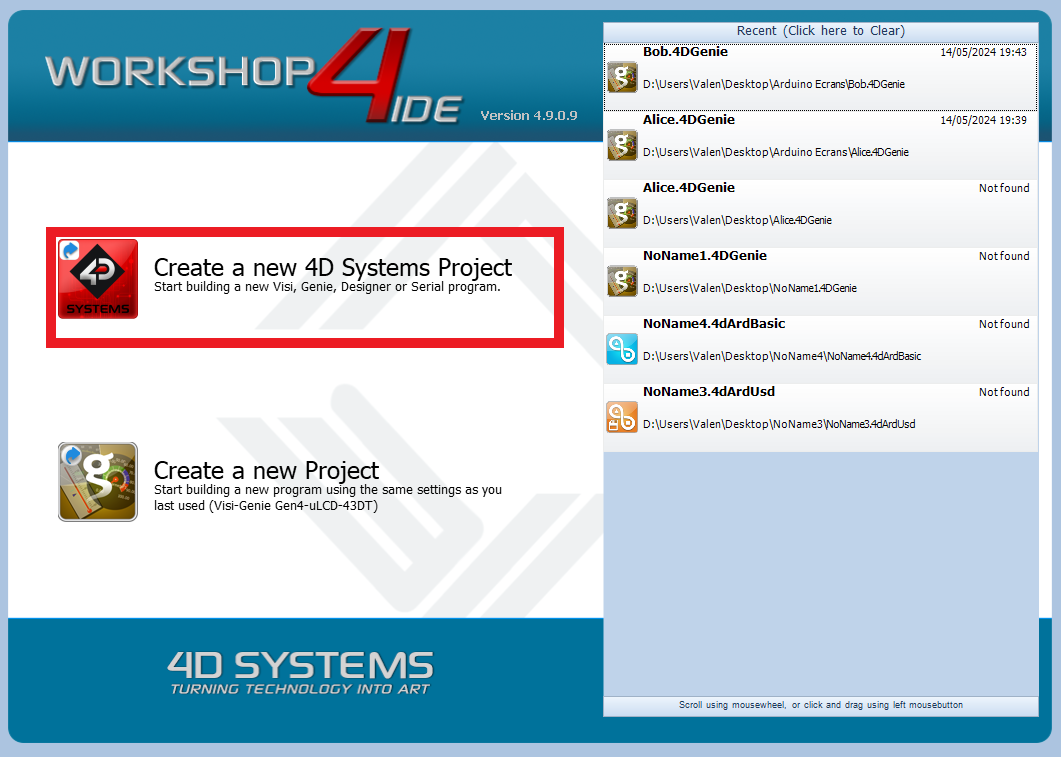
\includegraphics[width=\textwidth]{Format1.png}
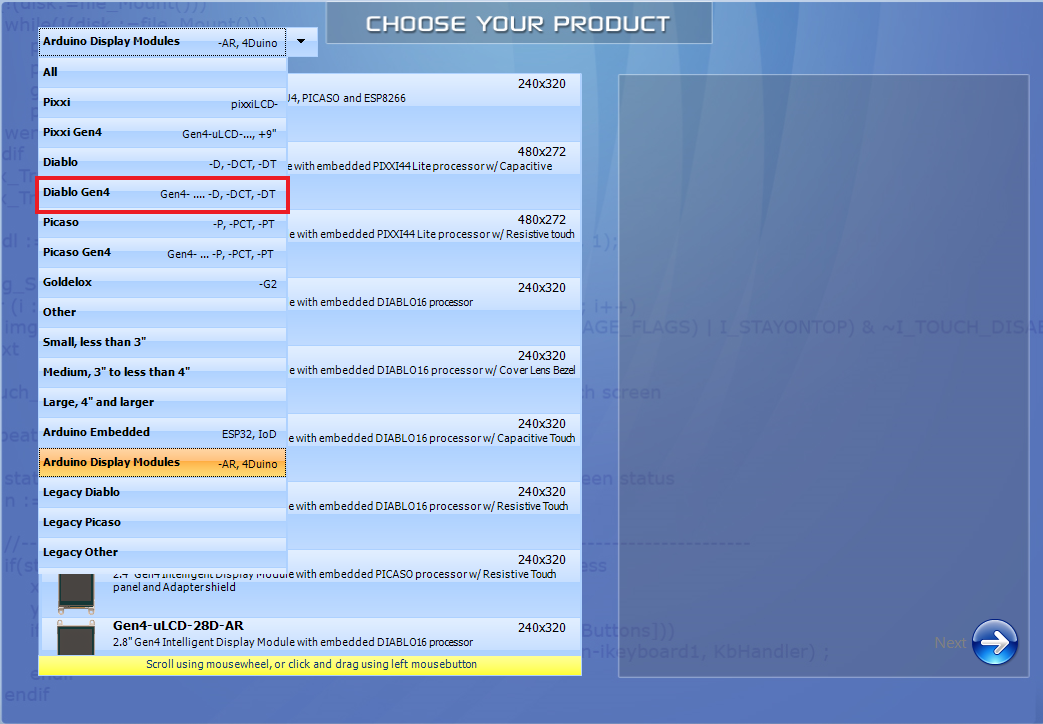
\includegraphics[width=\textwidth]{Format2.png}
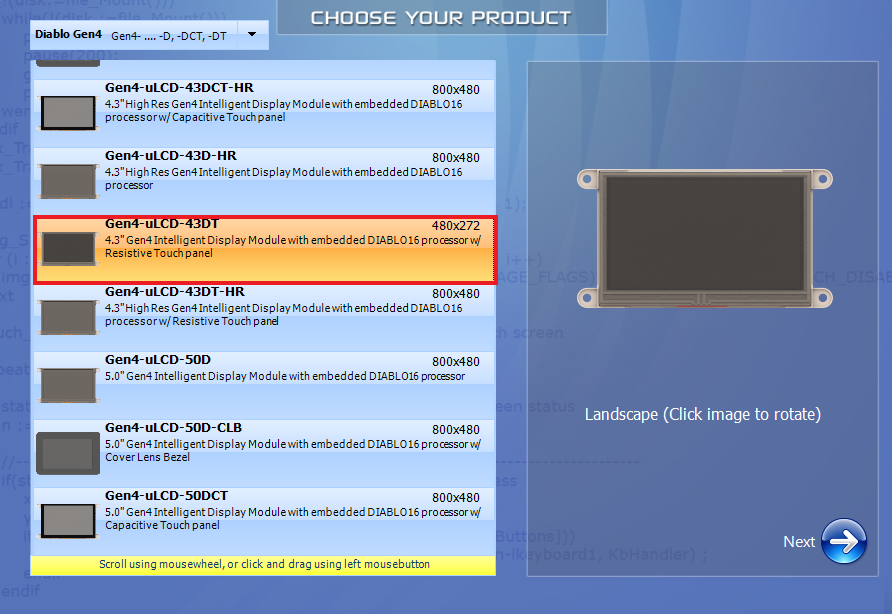
\includegraphics[width=\textwidth]{Format3.png}
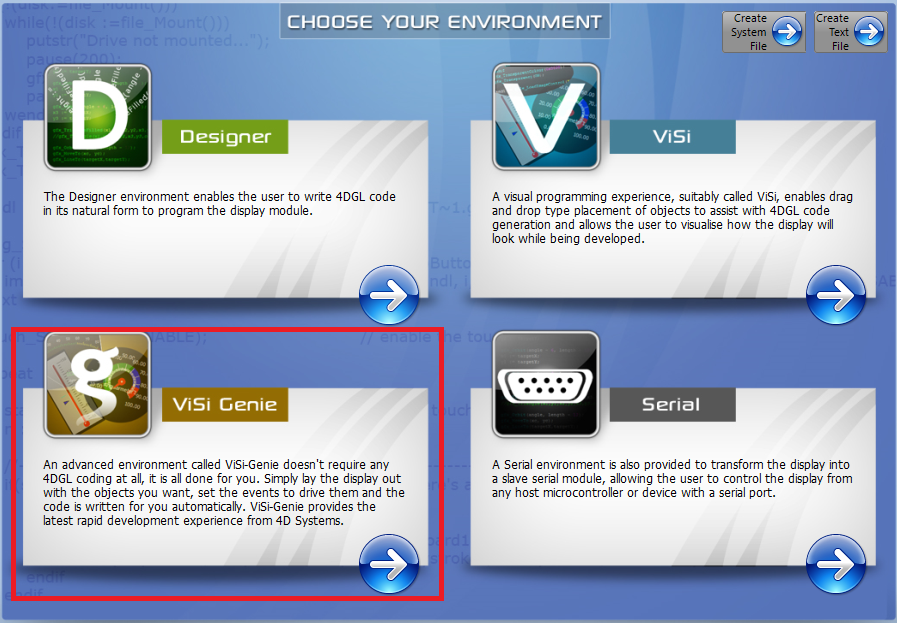
\includegraphics[width=\textwidth]{Format4.png}

\newpage
Une fois cela fait, il ne vous reste plus qu'à ouvrir l'outil PET dans les onglets supérieurs :

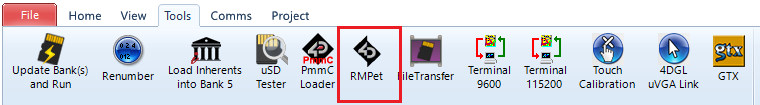
\includegraphics[width=\textwidth]{Format5.png}
\\

L'outil vous proposera de supprimer la table de partitions

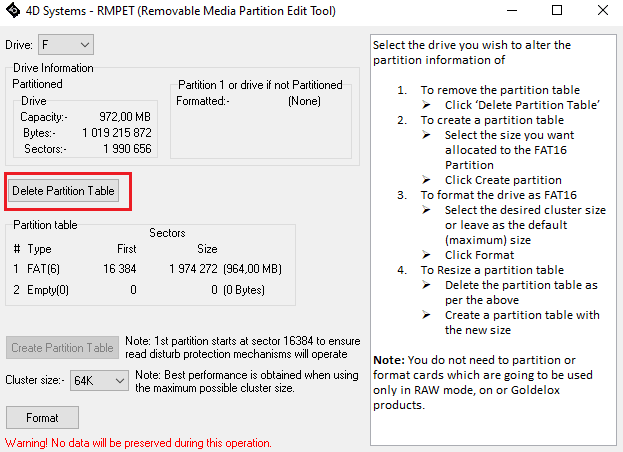
\includegraphics[width=\textwidth]{Format6.png}

Ensuite, vous les réallouez 

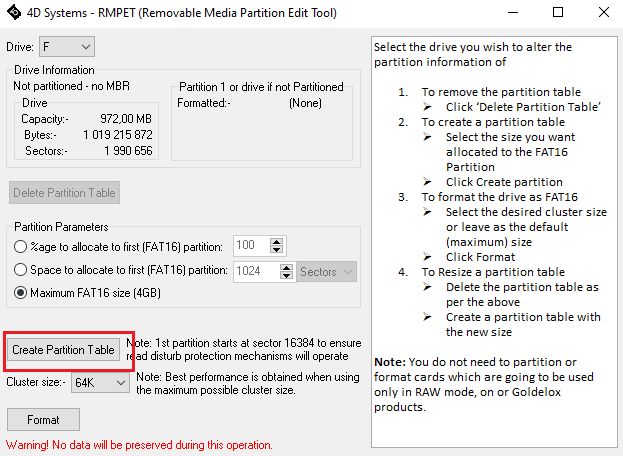
\includegraphics[width=\textwidth]{Format7.png}

Finalement, vous reformatez en FAT16 compatible 4DGénie

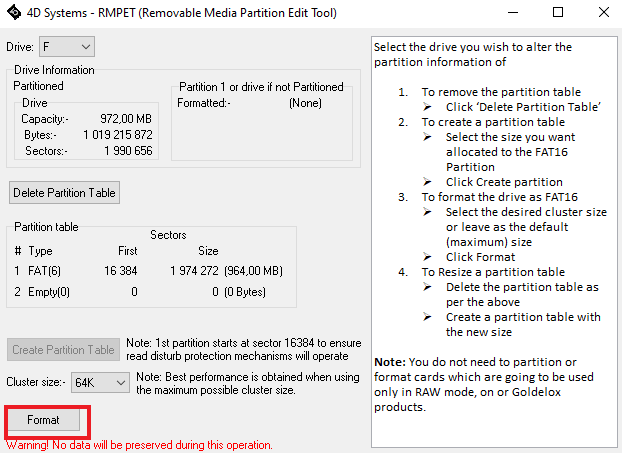
\includegraphics[width=\textwidth]{Format8.png}

Voilà ! La carte µSD est prête !

\newpage 
\subsubsection{Mise en place du code d'affichage}

Connectez l'écran à l'ordinateur, par le biais de l'adaptateur USB-A / Micro USB

Gardez la carte µSD branchée dans le lecteur de l'ordinateur, l'IDE Communique avec la carte µSD et l'écran sur deux canaux différents pour la première fois

Dans l'onglet COM, vérifiez que l'écran est reconnu. Sinon, déconnectez et reconnectez.
S'il est malgré tout pas reconnu, c'est probablement parce-que votre ordinateur ne dispose pas d'un pilote non obligatoire de détection des vieux périphériques, recherchez-en la version dans la section gestionnaire des périphériques de votre système d'exploitation.

Si votre écran est détecté, il vous faudra y télécharger des bibliothèques supplémentaires.
Dans l'onglet tools, sélectionnez l'option \emph{Load Inherents Into Bank 5}

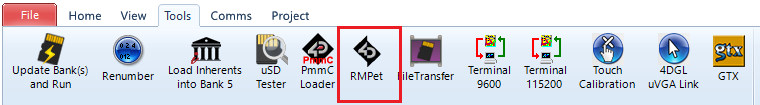
\includegraphics[width=\textwidth]{Format5.png}

Cela va télécharger des bibliothèques manquantes pour votre écran 

Une fois les bibliothèques installées, il ne vous reste plus qu'à transférer le code, en cliquant sur le bouton \emph{(Build) Copy/Load}, et vous sélectionnez la carte µSD.

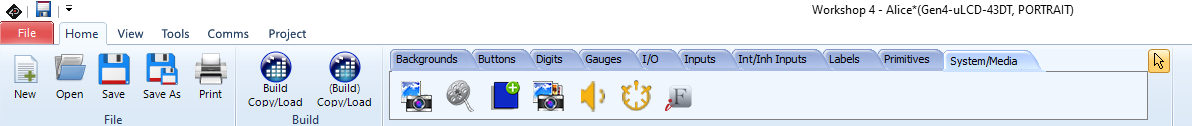
\includegraphics[width=\textwidth]{Transf1.png}

Une fois cela fait, vous réinsérez la carte µSD à l'arrière de l'écran.

Maintenant, l'écran est prêt !

\newpage

\section{Assemblage final de l'interface}

Une fois l'écran et l'Arduino prêts à l'usage, il ne vous reste plus qu'à monter l'écran et l'Arduino, comme suit :

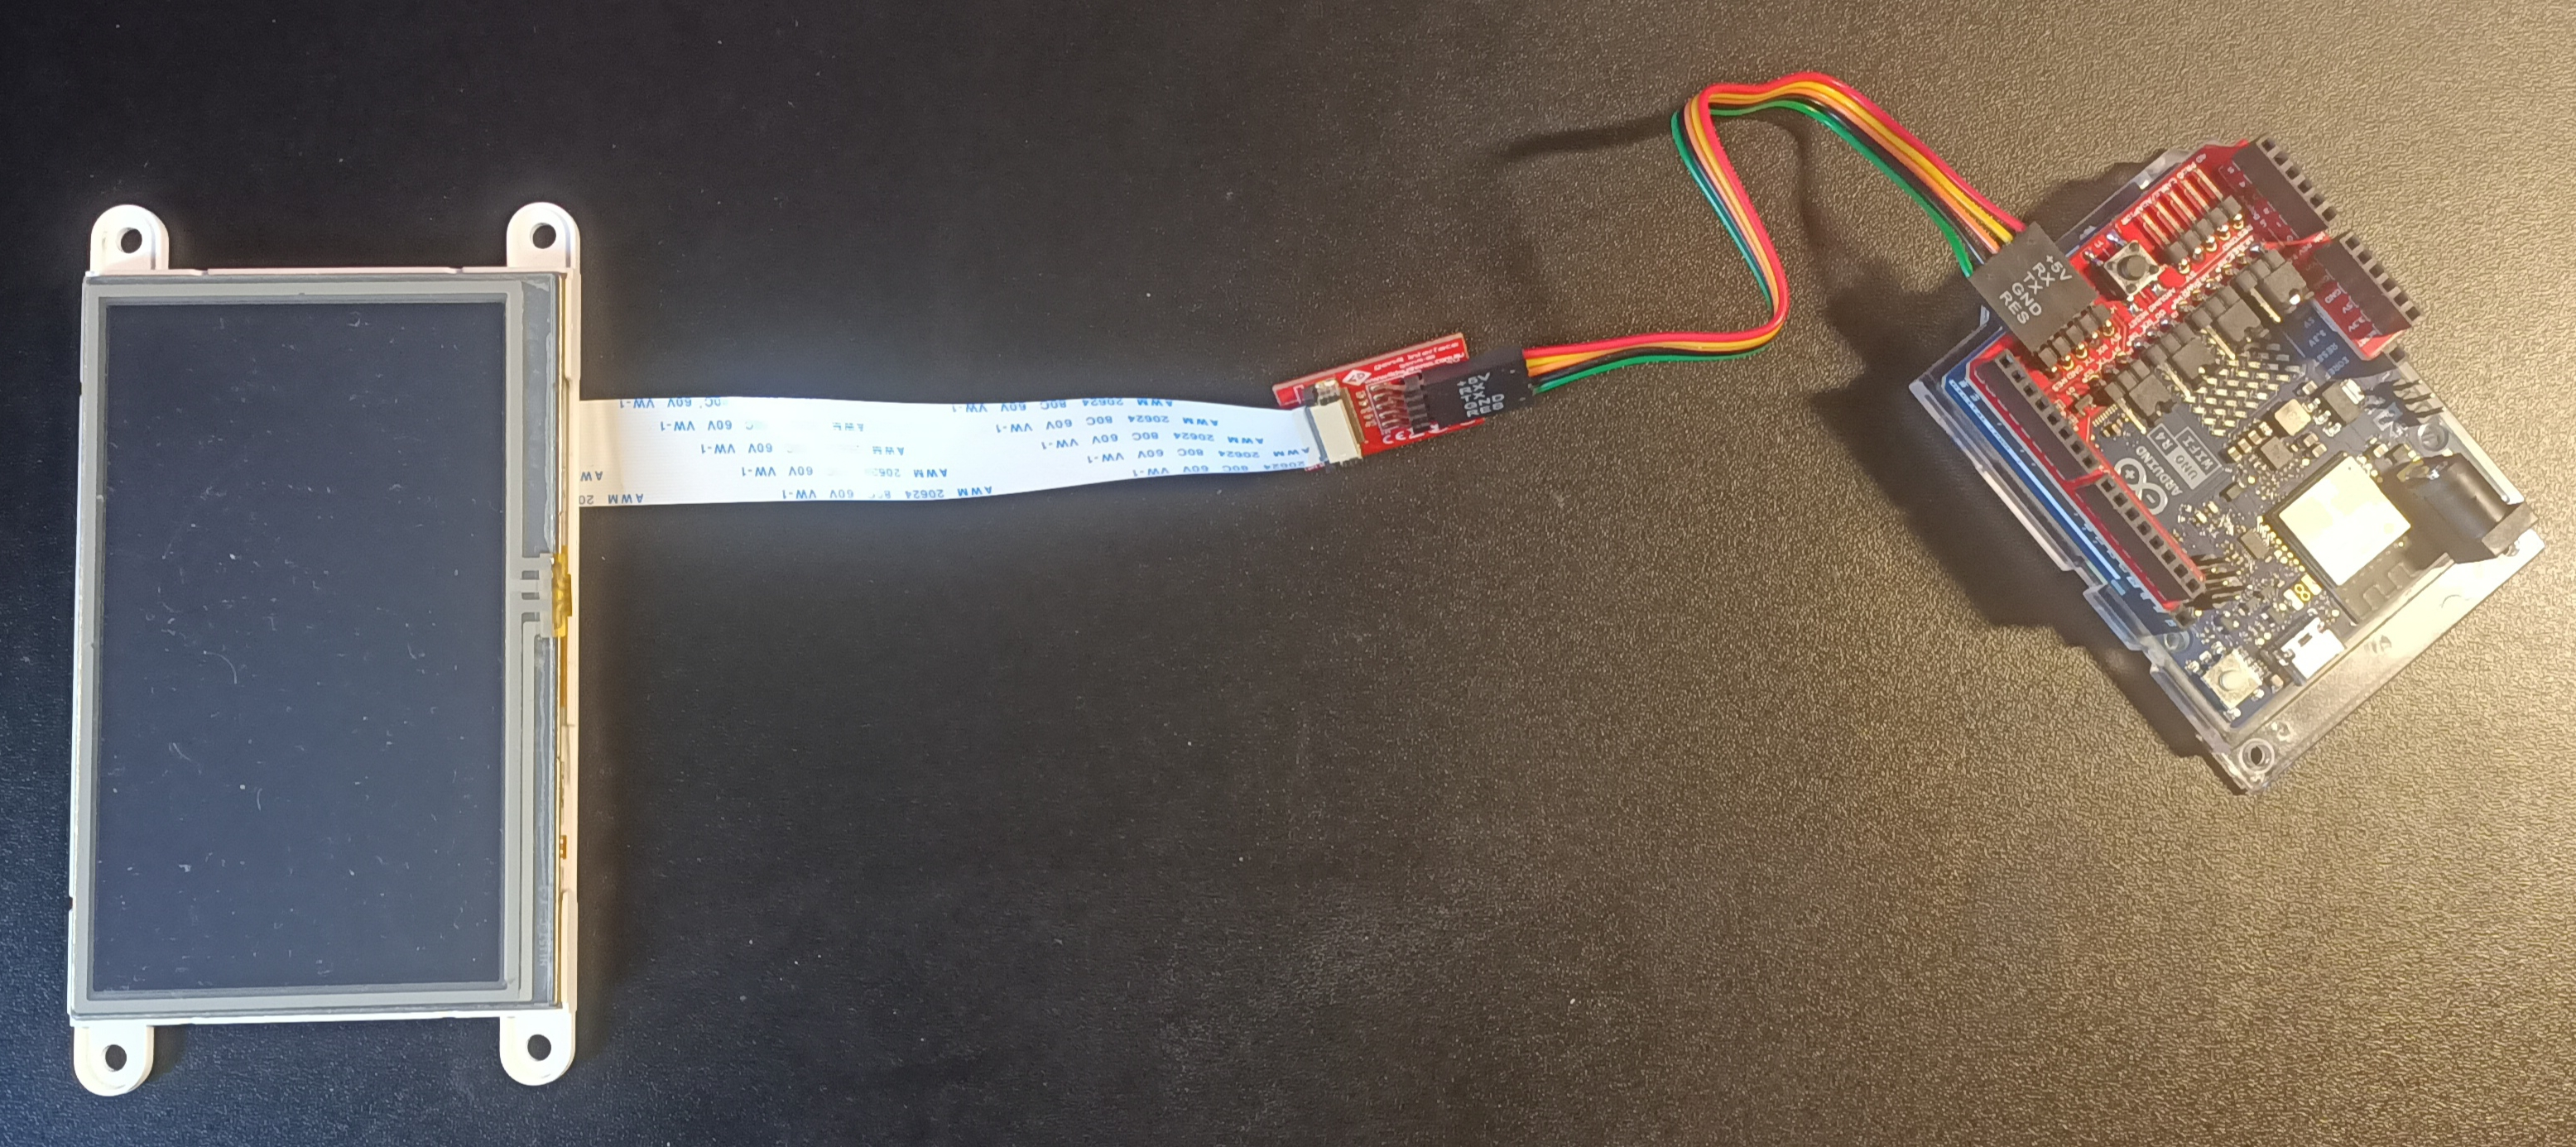
\includegraphics[width=\textwidth]{Appareil.jpg}

\end{document}